\chapter{Implementation Details}\label{chp:implementation}

Now we will look at some additional aspects of the practical implementations of the algorithms in previous chapters. Namely we will look at sparse multiplication and practical run time analysis of our nPoly library\cite{npoly}. Sparse multiplication is used when the number of non-zero terms in the polynomial proportion to the degree of the polynomial is low. The complexity of the algorithms we have covered so far have all been solely dependent on the degree of the polynomial and so these algorithms will perform poorly for sparse polynomials. Now we will look at a technique for sparse polynomial multiplication, this is also useful as it may be used as a base case for any of the algorithms we have covered here.

For example if we were to use Karatsuba's algorithm on $1 + x^2 + x^{60} + x^{100}$, then the algorithm would need to recurse $8$ times to reach a base case of one. However, if we organise our polynomial into a sparse vector and set a base case at $\# f \le 2$, then we only need to recurse once. Thus by formulating our base case in terms of the number of non-zero term in conduction with this algorithm, we may achieve a nice speedup. This algorithm also has the advantage for working equally over multivariate polynomials as well, which tend to be sparse in practice.

Note that this doesn't change the current complexity analysis from previous chapters as they were formulated to be independent of whether the coefficients were zero or non-zero, thus they used coefficient vector representations.

\section{Sparse Polynomial multiplication}

Previously in Chapter \ref{chp:classical} we showed that the schoolbook multiplication method has complexity $\M{O}(nm)$ for input polynomials of degree $n$ and $m$. However if our polynomials are reasonably sparse, it is natural to ask if we can design and algorithm with a complexity that is only dependent on the number of non-zero terms in the polynomial, rather than the maximum degree.

It would seem reasonable to try to use the schoolbook method to achieve this, however a problem arises when coordinating the access of elements in memory. Once we have multiplied two terms together, we need to include this result into the collection of terms we have calculated so far.

There are several methods we might look using to achieve this:
\begin{itemize}
    \item a coefficient vector. This requires potentially $\M{O}(n)$ time to shift data to allow the new term to be inserted,
    \item a binary tree would provide $\log n$ insertion times, but uses expensive memory operations and is not memory efficient, 
    \item a hashmap would provide $\M{O}(1)$ insertion time, but incurs additional costs when hashing the elements. Furthermore, since element in a hashmap are not store in any particular order, the elements would need to be sorted in the end, and so the complexity would be $m \log m$ where $m$ is the number of elements in the hashmap. This is more suitable in the case of multiplying many polynomials together as we then only need to sort the array once at the end.
\end{itemize}

Let $\# g$ denote the number of non-zero terms in the polynomial $g$. Say we are part way through multiplying two polynomials $a, b \in K[x]$. Denote the cumulative result after $k$ steps as $c_k$ e.g. after $\# a \# b$ steps we will have calculated the entire result so $c_{\#f + \#g} = ab$.

Using the formula
\[
    ab = \sum^{n + m}_{k=0} \bb{\sum_{i + j = k}a_ib_j} x^{i + j}.
\]
When we calculate another term $a_ib_j x^{i + j}$ for some $1 \le i \le n$ and $1 \le j \le m$, we now need add this to the resulting polynomial we have calculated so far. To find the matching monomial in our result polynomial (or insert it if it doesn't exist) we will need to perform a binary search. However, if we have stored the result as an array, then inserting the monomial could cause an $\#c_k$ shift in elements. If we store is as a linked list then this is not very efficient due to the expensive memory read operations.

Here I will present a technique for multiplying polynomials in $O(\# f \# g \log (\min\{\# f, \# g\})$. The main idea is to compute the monomials in order (as much as possible), so the output is naturally sorted. Later research found that this technique is similar to Johnson's sparse multiplication algorithm \cite{johnson-sparse-polynomial}.

As a practical example, we know that the smallest terms will be the lowest term of $f$ multiplied by the lowest term of $g$. Then the next smallest term in the result is either the smallest term of $f$ multiplied by the second smallest term of $g$, or vice versa. So we must compare them and output the smallest.

In general, fix a monomial order, then let $x_{ij}$ be the $i^{\text{th}}$ smallest monomial of $f$ multiplied by the $j^{\tx{th}}$ smallest monomial of $g$. Then $x_{ij} < x_{kj}$ when $k > i$ and $x_{ij} < x_{ik}$ when $k > j$. Thus before performing any calculations, we are able to deduce a partial ordering on the collection $\{x_{ij}\}_{i, j=0}^{i=\# f, j = \#g}$. The goal of the algorithm is to then resolve this into a total ordering in an efficient manner.

\begin{figure}
    \center
    \begin{tikzpicture}[baseline= (a).base]
        \node[scale=.8] (a) at (0,0){
                \begin{tikzcd}[column sep=small]
         & & & x_{\# f \# g} \arrow[ld] \arrow[rd] & & & \\
         & & x_{\# f (\# g - 1)} \arrow[ld] \arrow[rd] & & x_{(\# f - 1)\#g} \arrow[rd] \arrow[ld] & & \\
         & \cdots \arrow[ld] \arrow[rd] & & x_{(\# f - 1)(\# g - 1)} \arrow[rd] \arrow[ld] & & \cdots \arrow[rd] \arrow[ld] & \\
                    x_{\# f 1} \arrow[rd] & & \cdots \arrow[ld] \arrow[rd] & & \cdots \arrow[ld] \arrow[rd] & & x_{1 \# g} \arrow[ld] \\
                                          & \cdots \arrow[rd] & & x_{22} \arrow[rd] \arrow[ld] & & \cdots \arrow[ld] & \\
                                          & & x_{21} \arrow[rd] & & x_{12} \arrow[ld] & & \\
                                          & & & x_{11} & & &
                \end{tikzcd}
            };
    \end{tikzpicture}
    \caption{The partial order that is known a priori}
\end{figure}

The idea is that we start with $x_{ij}$ then we compute $x_{(i+1)j}$ and $x_{i(j+1)}$ and add them to the heap. We then take out the smallest and add it to the resulting vector. This is like starting from the $x_{11}$ and going up in the graph. In there is a path of arrows from one node to another, then that implies that node is definitely greater than it. It can then be seen from this graph that the most number of node that you can have in the heap at any time, occurs as a straight horizontal line across, which is $\min\{\# f, \# g\}$.


Therefore the multiplication operation will be $O(\# f \# g \min\{\# f, \# g\})$.


% \subsection{Sparse polynomial (my way)}

% The idea is that we compress the polynomial (i.e. ignoring the zero terms), then do a fft in that compressed state, multiply, then expand back into full
% e.g. Imagine $(x^{20} - 1)(x^{40} - 1)$, then I can replace the exponents with $n = 20$ and $m = 40$ and calculate $(x^n - 1)(x^m -1)$, which gives me $x^{n+m} - x^n - x^m + 1$, then I could have actually chosen $n = 1$ and $m = 2$, and calculated $(x - 1)(x^2 - 1)$ via the fft and gotten $x^3 - x^2 - x + 1$ and then expanded back into $x^{60} - x^{40} - x^{20} + 1$. Thats the basic premise

% I like the hybrid approach in the Fast Poly Mult paper. Also the mixed basis or small prime one

\section{Runtimes}

We have implemented several of the algorithms presented in this thesis as part of the nPoly polynomial arithmetic library. Rust is a modern systems programming language that has become increasingly popular in recent years for its ability to make highly-performant, highly generic code.

One of the advantages of Rust is its support for generic programming which has enabled nPoly to implement its algorithms over all algebras the algorithms support. Currently, nPoly supports: polynomial addition/subtraction/evaluation, Schoolbook multiplication, Karatsuba multiplication, FFT multiplication, Kronecker substitution and limited support for Gr\"{o}bner bases.

Here we will look at several algorithms, namely: Schoolbook multiplication (with hash-maps), Karatsuba's algorithm, and the standard FFT-based multiplication algorithm. One of the goals of this thesis was to develop a heuristic for selecting the most appropriate algorithm for a given set of input polynomials, however we note that the times obtained here are not highly optimised implementations as we have implemented all parts of the algorithms (including the FFT) ourselves. To improve the runtimes we may look at using existing software libraries to perform such parts of the code such as FFTW for the Fourier transform. Thus we can only explain the heuristic that nPoly uses for selecting its algorithms.

Beginning with the schoolbook method for multiplication, we have tested the algorithm by multiplying polynomials together with varying sparsity. We have also tested the runtime cost of increasing the number of indeterminates. As we can see, the number of indeterminates has a (roughly)-linear affect on the runtime performance, as we would expect since the only thing that would change is the hashing function used to hash the terms into the hash table. This hashing function is a source for potential optimisation as we have used the default function given by Rust, though since our monomials are vectors is $\Z^d$ (where $d$ is the number of indeterminates), it may be easy find more efficient hashing functions.

We also included a test for an optimised version of the univariate case. This involved a simpler monomial that the monomial data type we used for the other versions and is a bout two as faster when compared to the univariate case where we use the monomial for multi-indices type.

\begin{figure}[t]
    \centering
    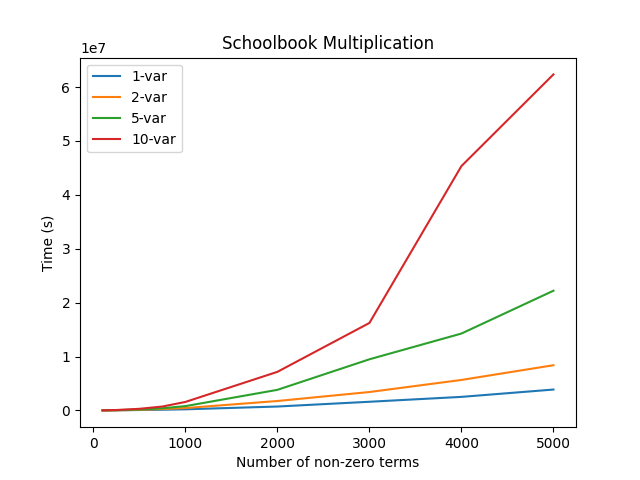
\includegraphics[width=12cm]{images/schoolbook-plot.pdf}
    \caption{Schoolbook Multiplication (hash-maps) on Sparse multivariate polynomials}
    \label{fig:schoolbook}
\end{figure}


As we can see, the FFT algorithm exhibits an $\M{O}(n \log n)$ complexity. Note however that it is measured in terms of the degrees of the input polynomials rather than the number of non-zero terms as the algorithm will behave the same regardless of the sparsity.

\begin{figure}[t]
    \centering
    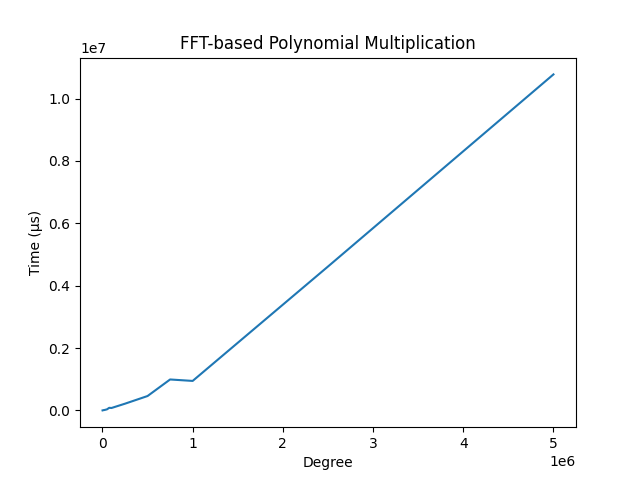
\includegraphics[width=12cm]{images/fft-plot.pdf}
    \caption{FFT-based polynomial multiplication algorithm on dense polynomials}
    \label{fig:fft}
\end{figure}

\begin{figure}[t]
    \centering
    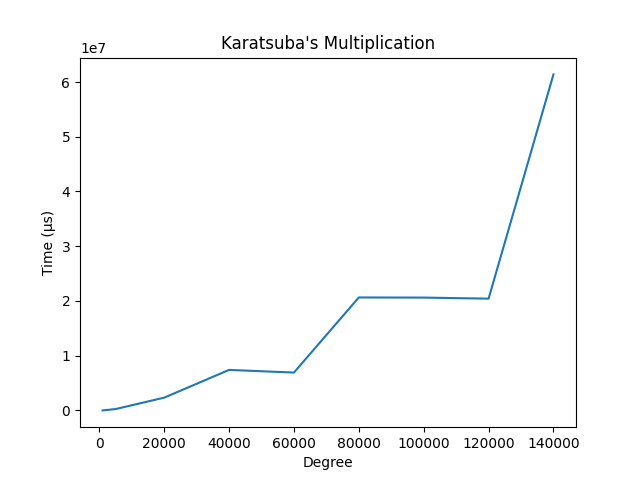
\includegraphics[width=12cm]{images/karatsuba-plot.pdf}
    \caption{Karatsuba's Algorithm for polynomial multiplication}
    \label{fig:karatsuba}
\end{figure}


We see here the runtime for a na\"{i}ve implementation of Kronecker substitution for converting multivariate polynomials to their univariate equivalent and back again. Note that this implementation creates new vectors each time and so it needs to dynamically allocate memory which may account for a significant proportion of the cost.

As we can see, Kronecker substitution performs quite poorly and has a similar complexity as the Schoolbook method. Thus we propose the optimisation as suggested in Section \ref{sub:implementation-kronecker} where we simply take a different algebraic meaning to the multi-indices to see them as univariate indices in a mixed-radix representation. This will incur no runtime costs if the polynomials are sorted in the lex order, however, we may need to reorganise the array of terms otherwise. This will be $\M{O}(n \log n)$ in the number of terms and so is insignificant compared to the cost of multiplication.

\begin{figure}[t]
    \centering
    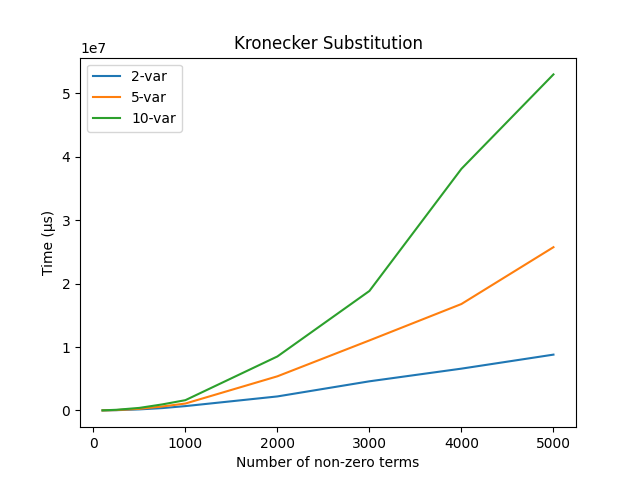
\includegraphics[width=12cm]{images/kronecker-plot.pdf}
    \caption{Na\"{i}ve Kronecker substitution on multivariate polynomials}
    \label{fig:kronecker}
\end{figure}


\begin{table}[h]
\centering
    \begin{tabular}{|c| c |}
        \hline
        Degree & time($\mu$s)\\
        \hline
        100 & 358\\
        1000 & 12516\\
        10000 & 772279\\
        100000 & 20829654\\
        200000 & 64446486\\
        \hline
    \end{tabular}
    \caption{Karatsuba's Algorithm}
\end{table}

\begin{table}[h]
\centering
    \begin{tabular}{|c| c |}
        \hline
        FFT & time($\mu$s)\\
        \hline
        100 & 92\\
        1000 & 544\\
        10000 & 7824\\
        100000 & 82067\\
        1000000 & 172875\\
        \hline
    \end{tabular}
    \caption{The FFT algorithm}
\end{table}

\begin{table}[h]
\centering
    \begin{tabular}{|c| c c c|}
        \hline
        Kronecker & 2 & 5 & 10\\
        \hline
        100 & 4153 & 5552 & 8891 \\
        250 & 28008 & 44412 & 68947 \\
        500 & 108576 & 177699 & 276068\\
        750 & 257015 & 414361 & 668346\\ 
        1000 & 419838 & 709191 & 1117284\\
        2500 & 2284089 & 5064354 & 9442733\\
        5000 & 6444083 & 19040990 & 65630087\\
        \hline
    \end{tabular}
    \caption{Na\"{i}ve Kronecker substitution}
\end{table}

\begin{table}[h]
\centering
    \begin{tabular}{|c| c c c c|}
        \hline
        Schoolbook & 1 & 2 & 5 & 10\\
        \hline
        100 & 2744 & 3280 & 4804 & 9731\\
        250 & 16879 & 32055 & 53999 & 75831\\
        500 & 74315 & 126403 & 168269 & 295479\\
        750 & 117782 & 268272 & 431288 & 730663\\
        1000 & 184860 & 428177 & 780056 & 1437264\\
        2500 & 1064871 & 2650782 & 5490774 & 10380380\\
        5000 & 4551621 & 8260184 & 22343481 & 66544669\\
        \hline
    \end{tabular}
    \caption{Schoolbook method with a hashmap}
\end{table}

\begin{table}[h]
\centering
    \begin{tabular}{|c| c |}
        \hline
        Schoolbook(optimised) & time($\mu$s)\\
        \hline
        100 & 1566 \\
        250 & 4906 \\
        500 & 14518 \\
        750 & 33088 \\
        1000 & 44487 \\
        2500 & 224304 \\
        5000 & 704417 \\
        \hline
    \end{tabular}
    \caption{Schoolbook method for univariate polynomials with an optimised monomial representation}
\end{table}


%%%%%%%%%%%%%%

% Karatsuba time(micro)
% 100 358
% 1000 12516
% 10000 772279
% 100000 20829654
% 200000 64446486

% FFT time(nano)
% 100 92892
% 1000 544623
% 10000 7824356
% 100000 82067888
% 1000000 172875383
% 2000000 1233622640

% Kronecker two five ten
% 100  4153   5552      8891 
% 250  28008  44412     68947 
% 500  108576 177699    276068 
% 750  257015 414361    668346 
% 1000 419838  709191   1117284 
% 2500 2284089 5064354  9442733 
% 5000 6444083 19040990 65630087

% Schoolbook (uni) two five ten
% 100 2744     3280     4804      9731     
% 250 16879    32055    53999     75831    
% 500 74315    126403   168269    295479   
% 750 117782   268272   431288    730663   
% 1000 184860  428177   780056    1437264  
% 2500 1064871 2650782  5490774   10380380  
% 5000 4551621 8260184  22343481  66544669  


% Schoolbook(uni-optimised) time(micro)
% 100 1566 
% 250 4906 
% 500 14518 
% 750 33088 
% 1000 44487 
% 2500 224304 
% 5000 704417 
% \subsection{Sparse evaluation}

% So i've got an algorithm here for some sparse multiplication technique.

% The basic premise is that we consider the tree created by the FFT and then we want to cut off branches, but by ``cut off'' I mean, ``never actually create in the first place''. So to do that we do as follows

% Construct the tree below.
% Then we add the elements in their reverse bit order. When we add an element, we slide it down the tree as far right as possible. All the ones that slide to the left need to have a calculation first.

% Note: We can probably leverage the intermediate results from the bucket sort, for instance, if one bucket is empty after the first pass, then we know that that subtree is actually empty. So if the bucket sort is inefficient, then actually that implies that your underlying data in not random and can actually be leveraged because you know whole subtrees will be empty

% \begin{algorithm}[H]
%     \SetAlgoLined
%     \KwData{Vector of monomials to be transformed (non-expanded)}
%     \KwResult{Fourier transform of the input coefficients}
%     rbe $\gets$ Reverse Bit Encoding of monomials\;
%     acc $\gets$ Empty vector\;
%     \For{el in rbe}{
%         acc.push(el)\;
%         \While{acc.len() > 1 \&\& canCombine(acc[-2], acc[-1])}{
%             tmp $\gets$ acc.pop()\;
%             acc[-1].combine(tmp)\;
%         }
%     }
%     \Return{acc}
%     \caption{Sparse FFT}
% \end{algorithm}


% \begin{algorithm}[H]
%     \SetAlgoLined
%     \KwData{arg1, arg2: Two subtrees}
%     \KwResult{Boolean}
%     depth $\gets$ findLowestConnection(arg1.path, arg2.path, arg1.depth, arg2.depth)\;
%     \Comment{Note that simply constructing such a number of all 1's and testing if equal would be quicker}\;
%     \For{i in 0 ... (node - arg2.index)}{
%         \If{arg2.index \& 1 $<<<$ i = 0}{
%             \Return false
%         }
%     }
%     \Return{true}
%     \caption{canCombine}
% \end{algorithm}

% \begin{algorithm}[H]
%     \SetAlgoLined
%     \KwData{path1, path2: Two subtrees; depth1, depth2: Usize}
%     \KwResult{Absolute depth of the connecting tree: usize}
%     \eIf{depth1 > depth2}{
%         path2 >>= depth1 - depth2\;
%         depth2 = depth1
%         }{
%         path1 >>= depth2 - depth1\;
%         depth1 = depth2
%     }
%     count $\gets$ 0\;
%     \While{path1 $\neq$ path2}{
%         count += 1\;
%         path1 >>= 1\;
%         path2 >>= 1\;
%     }
%     \Return{count + depth}
%     \caption{findLowestConnection}
% \end{algorithm}

% \begin{enumerate}[1.]
%     \item Organise the list into its Reverse Bit encoding ($O(t \log t \log n)$). The $\log n$ term arises from the degrees of the polynomials are literally have $\log n$ space complexity
%     \item Add a new element to the vector and see if it can be combined with the previous element or we need to wait to see if it needs to be combined with the next element first
%     \item To combine, we ``expand'' the two elements into the appropriate size and then do the combination step from the FFT
%     \item Continue until all the elements have gone
%     \item Finish by combining all the elements remaining in the list into the final transform
% \end{enumerate}

% Unfortunately in this one we still end up expanding the polynomials in the end so it must be $O(n\log n)$. But we should try not to do that.\\
% The best result would be if I could interpolate the results whilst still in their $O(t)$ space complexity format. Then we would also have a good representation for our resulting polynomial if we wanted to do calculations based on that.

% \section{Search trees for membership in monomial ideals}

% \textbf{Problem:} Given a monomial ideal, want to test to see if a monomial is in it.

% The time to beat is $O(nm)$ where $n$ is the number of generators in the ideal and $m$ is the number of indeterminates. This is obtained by a linear search

% The next best thing would be to try and do a search based off each of the values in the multi-index. You would try to do a binary search on th first value, then on the second, and so on. The problem is that it is pretty hard to see what kind of data structure this might use.

% Another optimisation would be to record the highest index value for each of the indices. Then we might be able to fit multiple indices inside a single machine word.

% The division relation "|", where $a | b$ for $a$ and $b$ monomials. Is independent of monomial orderings, and is reflexive and transitive. But it is not a total order so we cannot perform a normal binary search. In fact, if we have that one generator of the ideal divides the other, then the other can be eliminated so it is unclear how we would even go about searching for divisibility.

% What we can do is:
% \begin{enumerate}
%     \item Order then by total degree, if $\tx{totdeg}(a) < \tx{totdeg}(b)$ then certainly $b \not | a$. This can give us a rough estimate of where to place it
%     \item Order by total degree of the first half of the multi-index. Say if we have a monomial with multi-index $(1, 0, 5, 6, 2, 4)$, then we have its total degree is $1 + 5 + 6 + 2 + 4 = 18$, then the total degree of the first half is $1 + 0 + 5 = 6$.
%     \item Then order by their second half and so forth. This way we can build up a key for the monomial.
% \end{enumerate}

% This still has some of the same problems as the previous method of just searching through the indices but I think on average it will be quicker because the variance in the variables should be lower when you sum them and so they should be more accurate.

% Actually I would propose this as a new monomial order. It might allow you to obtain tighter bounds on certain algorithms.
